\definecolor{white}{rgb}{1.0, 1.0, 1.0}
\clearpage
\section{Suddivisione risorse e preventivi}
\label{sec:sud_risorse_preve}
La suddivisione oraria viene fatta tenendo conto delle seguenti regole:
\begin{enumerate}
\item Ogni membro a rotazione deve coprire ogni ruolo almeno una volta
\item Ogni membro dovrà lavorare almeno 6 ore per ogni figura di progetto in modo da apprendere a pieno i compiti che ciascun ruolo richiede
\item Il monte ore totale del lavoro di ciascun membro dovrà essere uguale oppure differire di qualche ora
\end{enumerate}
Le ore investite durante il periodo relativo all'Analisi non verranno conteggiate nelle ore totali da retribuire. Questo tempo non viene considerato da \textit{duckware} come a carico del committente.
\clearpage
\subsection{Analisi}
\label{sec:periodo_analisi}
\subsubsection{Prospetto orario}
La seguente è la distribuzione oraria durante il periodo di Analisi:
\begin{center}
	\renewcommand{\arraystretch}{1.5}
	\rowcolors{3}{tableLightYellow}{}
	\begin{longtable}[H]{ 	>{\RaggedRight}p{3.5cm}  
							>{\Centering}p{1.2cm} 
							>{\Centering}p{1.2cm}  
							>{\Centering}p{1.2cm} 
							>{\Centering}p{1.2cm}  
							>{\Centering}p{1.2cm} 
							>{\Centering}p{1.2cm}  
							>{\Centering}p{1.4cm}  
							}
		\rowcolor{tableHeadYellow}
		\textbf{Nome}   & \textbf{Re} & \textbf{Ad} & \textbf{An} & \textbf{Pj} & \textbf{Pr} & \textbf{Ve} & \textbf{TOT} \\ 
		\endhead
		
		Luca Stocco       & 0   & 10    & 5   & 0   & 0   & 10 	& 25 \\  
		Alberto Miola     & 3   & 10    & 4   & 0   & 0   & 8  	& 25 \\  
		Andrea Pavin      & 3  	& 5     & 12  & 0   & 0   & 8  	& 28 \\  
		Sonia Menon       & 4  	& 9     & 3   & 0   & 0   & 10  & 26 \\  
		Pardeep Singh     & 8   & 2     & 10  & 0   & 0   & 4  	& 24 \\  
		Matteo Pellanda   & 4   & 8     & 7   & 0   & 0   & 3 	& 22 \\
		Alessandro Pegoraro	& 0	& 10	& 9	  & 0	& 0	  & 6	& 25\\
		
		\rowcolor{white}
		\caption{Tabella prospetto orario}
	\end{longtable}
\end{center}
Il seguente grafico mostra visivamente la suddivisione oraria:
%(immagine grafico 1)
\begin{figure}[H]
	\centering
	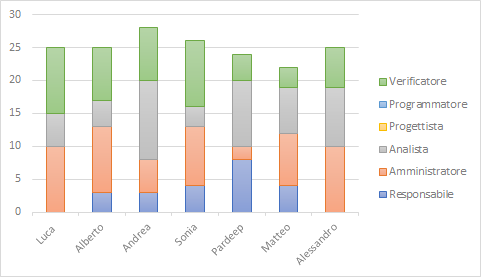
\includegraphics[width=15cm,keepaspectratio]{../includes/pics/grafici/grafico1.png}
	\caption{\label{fig:mission}Divisione dei ruoli tra i membri}
\end{figure}
\clearpage
\subsubsection{Prospetto economico}
Durante il periodo di analisi la distribuzione dei ruoli fra i membri del gruppo è stata la seguente:
\begin{center}
	\renewcommand{\arraystretch}{1.5}
	\rowcolors{3}{tableLightYellow}{}
	\begin{longtable}[H]{  	>{\RaggedRight}p{5.6cm}  
							>{\RaggedRight}p{3cm} 
							>{\RaggedRight}p{3cm}  
							}
		\rowcolor{tableHeadYellow}
		\textbf{Ruolo}   & \textbf{Ore} & \textbf{Costo (Euro)} \\ 
		\endhead
		Responsabile   & 22   & 660,00 \euro \\
		Amministratore & 54   & 1.080,00 \euro \\
		Analista       & 50   & 1.250,00 \euro\\
		Progettista    & 0    & 0,00 \euro \\
		Programmatore  & 0    & 0,00 \euro \\
		Verificatore   & 49   & 735,00 \euro\\
		Totale         & 175   & 3.725,00 \euro \\
		\rowcolor{white}
		\caption{Tabella prospetto economico}
	\end{longtable}
\end{center}
Il seguente grafico mostra visivamente la distribuzione dei ruoli:
%(immagine grafico 2)
\begin{figure}[H]
	\centering
	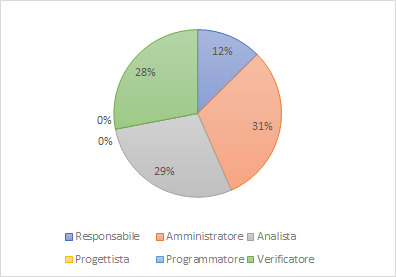
\includegraphics[width=15cm,keepaspectratio]{../includes/pics/grafici/grafico2.png}
	\caption{\label{fig:mission}Distribuzione oraria dei ruoli}
\end{figure}
\clearpage
\subsection{Consolidamento dei requisiti}
\label{sec:consolidamento_requisiti}
\subsubsection{Prospetto orario}
Durante il periodo di consolidamento la distribuzione oraria fra i membri del gruppo è stata la seguente:
\begin{center}
	\renewcommand{\arraystretch}{1.5}
	\rowcolors{3}{tableLightYellow}{}
	\begin{longtable}[H]{ 	>{\RaggedRight}p{3.5cm}  
							>{\Centering}p{1.2cm} 
							>{\Centering}p{1.2cm}  
							>{\Centering}p{1.2cm} 
							>{\Centering}p{1.2cm}  
							>{\Centering}p{1.2cm} 
							>{\Centering}p{1.2cm}  
							>{\Centering}p{1.4cm}  
							}
		\rowcolor{tableHeadYellow}
		\textbf{Nome}   & \textbf{Re} & \textbf{Ad} & \textbf{An} & \textbf{Pj} & \textbf{Pr} & \textbf{Ve} & \textbf{TOT} \\ 
		\endhead
		
		Luca Stocco       & 6   & 1     & 0   & 0   & 0   & 0  &    7 \\  
		Alberto Miola     & 0   & 2     & 0   & 0   & 0   & 5  &    7 \\  
		Andrea Pavin      & 0   & 0     & 4   & 0   & 0   & 3  &    7 \\  
		Sonia Menon       & 0   & 5     & 2   & 0   & 0   & 0  &    7 \\  
		Pardeep Singh     & 0   & 0     & 0   & 0   & 0   & 7  &    7 \\  
		Matteo Pellanda   & 0   & 0     & 7   & 0   & 0   & 0  &    7 \\
		Alessandro Pegoraro & 0 & 2 	& 3   &	0	& 0	  & 2 	& 7 \\ 

		\rowcolor{white}
		\caption{Tabella prospetto orario}
	\end{longtable}
\end{center}
Il seguente grafico mostra visivamente la distribuzione dei ruoli:
%(immagine grafico 3)
\begin{figure}[H]
	\centering
	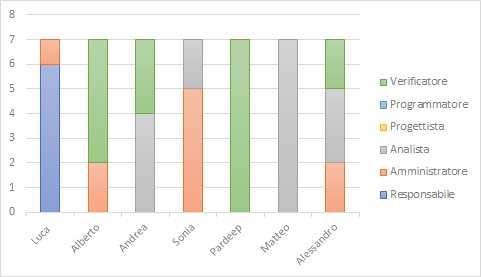
\includegraphics[width=15cm,keepaspectratio]{../includes/pics/grafici/grafico3.png}
	\caption{\label{fig:mission}Divisione dei ruoli tra i membri}
\end{figure}
\clearpage
\subsubsection{Prospetto economico}
Durante il periodo di consolidamento la distribuzione dei ruoli fra i membri del gruppo è stata la seguente:
\begin{center}
	\renewcommand{\arraystretch}{1.5}
	\rowcolors{3}{tableLightYellow}{}
	\begin{longtable}[H]{  	>{\RaggedRight}p{5.6cm}  
							>{\RaggedRight}p{3cm} 
							>{\RaggedRight}p{3cm}  
							}
		\rowcolor{tableHeadYellow}
		\textbf{Ruolo}   & \textbf{Ore} & \textbf{Costo (Euro)} \\ 
		\endhead

		Responsabile   & 6    & 180,00 \\
		Amministratore & 10    & 160,00 \\
		Analista       & 16   & 325,00 \\
		Progettista    & 0    & 0,00 \\
		Programmatore  & 0    & 0,00 \\
		Verificatore   & 17   & 225,00 \\
		Totale         & 49   & 890,00 \\

		\rowcolor{white}
		\caption{Tabella prospetto economico}
	\end{longtable}
\end{center}
Il seguente grafico mostra visivamente la distribuzione dei ruoli:
%(immagine grafico 4)
\begin{figure}[H]
	\centering
	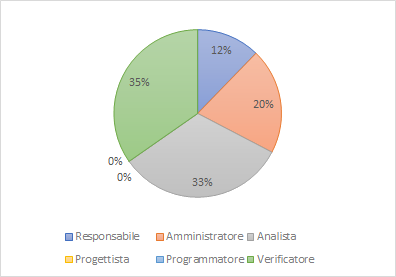
\includegraphics[width=15cm,keepaspectratio]{../includes/pics/grafici/grafico4.png}
	\caption{\label{fig:mission}Divisione dei ruoli tra i membri}
\end{figure}
\clearpage
\subsection{Progettazione base tecnologica}
\label{sec:progettazione_base_tecnologica}
\subsubsection{Prospetto orario}
Durante il periodo di progettazione di base la distribuzione oraria fra i membri del gruppo è stata la seguente:
\begin{center}
	\renewcommand{\arraystretch}{1.5}
	\rowcolors{3}{tableLightYellow}{}
	\begin{longtable}[H]{ 	>{\RaggedRight}p{3.5cm}  
							>{\Centering}p{1.2cm} 
							>{\Centering}p{1.2cm}  
							>{\Centering}p{1.2cm} 
							>{\Centering}p{1.2cm}  
							>{\Centering}p{1.2cm} 
							>{\Centering}p{1.2cm}  
							>{\Centering}p{1.4cm}  
							}
		\rowcolor{tableHeadYellow}
		\textbf{Nome}   & \textbf{Re} & \textbf{Ad} & \textbf{An} & \textbf{Pj} & \textbf{Pr} & \textbf{Ve} & \textbf{TOT} \\ 
		\endhead

		Luca Stocco       & 7   & 0     & 2 	& 8		& 4 	& 12  	& 33 \\  
		Alberto Miola     & 0   & 0     & 4  	& 8  	& 12   	& 5  	& 29 \\  
		Andrea Pavin      & 6   & 7     & 0   	& 6  	& 5   	& 10  	& 34 \\  
		Sonia Menon       & 0   & 4     & 2   	& 6   	& 8  	& 11 	& 31 \\  
		Pardeep Singh     & 0   & 3     & 0   	& 10  	& 4  	& 10 	& 27 \\  
		Matteo Pellanda   & 3   & 0     & 2  	& 6   	& 7   	& 9  	& 27 \\ 
		Alessandro Pegoraro & 0 & 4		& 3		& 7		&6 		& 7 	& 27\\  

		\rowcolor{white}
		\caption{Tabella prospetto orario}
	\end{longtable}
\end{center}
Il seguente grafico mostra visivamente la distribuzione dei ruoli:
%(immagine grafico 5)
\begin{figure}[H]
	\centering
	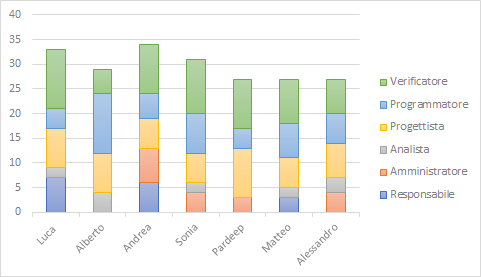
\includegraphics[width=15cm,keepaspectratio]{../includes/pics/grafici/grafico5.png}
	\caption{\label{fig:mission}Distribuzione oraria dei ruoli}
\end{figure}
\clearpage
\subsubsection{Prospetto economico}
Durante il periodo di progettazione di base la distribuzione dei ruoli fra i membri del gruppo è stata la seguente:
\begin{center}
	\renewcommand{\arraystretch}{1.5}
	\rowcolors{3}{tableLightYellow}{}
	\begin{longtable}[H]{  	>{\RaggedRight}p{5.6cm}  
							>{\RaggedRight}p{3cm} 
							>{\RaggedRight}p{3cm}  
							}

		\rowcolor{tableHeadYellow}
		\textbf{Ruolo}   & \textbf{Ore} & \textbf{Costo (Euro)} \\ 
		\endhead

		Responsabile   & 16   & 480,00 \\
		Amministratore & 18   & 360,00 \\
		Analista       & 13   & 325,00 \\
		Progettista    & 51   & 1.122,00 \\
		Programmatore  & 40   & 600,00 \\
		Verificatore   & 64   & 960,00 \\
		Totale         & 202  & 3.847,00 \\

		\rowcolor{white}
		\caption{Tabella prospetto economico}
	\end{longtable}
\end{center}
Il seguente grafico mostra visivamente la distribuzione dei ruoli:
%(immagine grafico 6)
\begin{figure}[H]
	\centering
	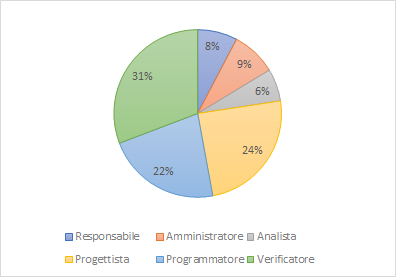
\includegraphics[width=15cm,keepaspectratio]{../includes/pics/grafici/grafico6.png}
	\caption{\label{fig:mission}Divisione dei ruoli tra i membri}
\end{figure}
\clearpage
\subsection{Progettazione di dettaglio e codifica}
\label{sec:progettazione_dettaglio_codifica}
\subsubsection{Prospetto orario}
Durante il periodo di progettazione di dettaglio e codifica la distribuzione oraria fra i membri del gruppo è stata la seguente:
\begin{center}
	\renewcommand{\arraystretch}{1.5}
	\rowcolors{3}{tableLightYellow}{}
	\begin{longtable}[H]{ 	>{\RaggedRight}p{3.5cm}  
							>{\Centering}p{1.2cm} 
							>{\Centering}p{1.2cm}  
							>{\Centering}p{1.2cm} 
							>{\Centering}p{1.2cm}  
							>{\Centering}p{1.2cm} 
							>{\Centering}p{1.2cm}  
							>{\Centering}p{1.4cm}  
							}
							
		\rowcolor{tableHeadYellow}
		\textbf{Nome}   & \textbf{Re} & \textbf{Ad} & \textbf{An} & \textbf{Pj} & \textbf{Pr} & \textbf{Ve} & \textbf{TOT} \\ 
		\endhead

		Luca Stocco       & 0   & 4     & 0   & 16   & 17   & 8   	& 45 \\  
		Alberto Miola     & 5   & 5     & 0   & 15   & 11   & 13  	& 49 \\  
		Andrea Pavin      & 0   & 0     & 3   & 16   & 17   & 10  	& 46 \\  
		Sonia Menon       & 0   & 0     & 0   & 16   & 16   & 12  	& 44 \\  
		Pardeep Singh     & 3   & 4     & 4   & 16   & 15   & 11  	& 53 \\  
		Matteo Pellanda   & 0   & 4     & 3   & 18   & 14   & 10  	& 49 \\
		Alessandro Pegoraro & 7 & 3		& 2	  & 17	 & 13	& 11 	& 53 \\   

		\rowcolor{white}
		\caption{Tabella prospetto orario}
	\end{longtable}
\end{center}
Il seguente grafico mostra visivamente la distribuzione dei ruoli:
%(immagine grafico 7)
\begin{figure}[H]
	\centering
	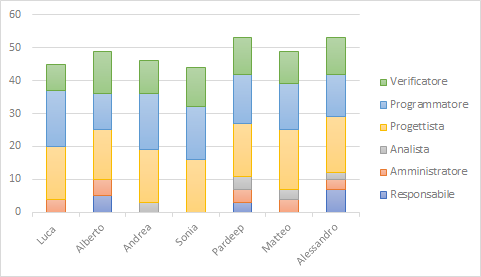
\includegraphics[width=15cm,keepaspectratio]{../includes/pics/grafici/grafico7.png}
	\caption{\label{fig:mission}Distribuzione oraria dei ruoli}
\end{figure}
\clearpage
\subsubsection{Prospetto economico}
Durante il periodo di progettazione di dettaglio e codifica la distribuzione dei ruoli fra i membri del gruppo è stata la seguente:
\begin{center}
	\renewcommand{\arraystretch}{1.5}
	\rowcolors{3}{tableLightYellow}{}
	\begin{longtable}[H]{  	>{\RaggedRight}p{5.6cm}  
							>{\RaggedRight}p{3cm} 
							>{\RaggedRight}p{3cm}  
							}

		\rowcolor{tableHeadYellow}
		\textbf{Ruolo}   & \textbf{Ore} & \textbf{Costo (Euro)} \\ 
		\endhead

		Responsabile   & 15   & 450,00 \\
		Amministratore & 20   & 400,00 \\
		Analista       & 12   & 300,00 \\
		Progettista    & 114  & 2.508,00 \\
		Programmatore  & 103  & 1.545,00 \\
		Verificatore   & 75   & 1.125,00 \\
		Totale         & 339  & 6.328,00 \\

		\rowcolor{white}
		\caption{Tabella prospetto economico}
	\end{longtable}
\end{center}
Il seguente grafico mostra visivamente la distribuzione dei ruoli:
%(immagine grafico 8)
\begin{figure}[H]
	\centering
	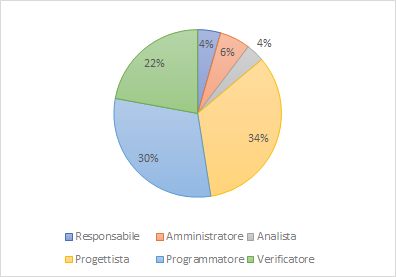
\includegraphics[width=15cm,keepaspectratio]{../includes/pics/grafici/grafico8.png}
	\caption{\label{fig:mission}Divisione dei ruoli tra i membri}
\end{figure}
\clearpage
\subsection{Validazione e collaudo}
\label{sec:validazione_collaudo}
\subsubsection{Prospetto orario}
Durante il periodo di \markg{validazione} la distribuzione oraria fra i membri del gruppo è stata la seguente:
\begin{center}
	\renewcommand{\arraystretch}{1.5}
	\rowcolors{3}{tableLightYellow}{}
	\begin{longtable}[H]{ 	>{\RaggedRight}p{3.5cm}  
							>{\Centering}p{1.2cm} 
							>{\Centering}p{1.2cm}  
							>{\Centering}p{1.2cm} 
							>{\Centering}p{1.2cm}  
							>{\Centering}p{1.2cm} 
							>{\Centering}p{1.2cm}  
							>{\Centering}p{1.4cm}  
							}
							
		\rowcolor{tableHeadYellow}
		\textbf{Nome}   & \textbf{Re} & \textbf{Ad} & \textbf{An} & \textbf{Pj} & \textbf{Pr} & \textbf{Ve} & \textbf{TOT} \\ 
		\endhead

		Luca Stocco       & 0   & 4     & 0   & 6    & 6    & 6   	& 22 \\  
		Alberto Miola     & 0   & 4     & 0   & 8    & 4    & 6   	& 22 \\  
		Andrea Pavin      & 0   & 3     & 0   & 6    & 5    & 6   	& 20 \\  
		Sonia Menon       & 10  & 3     & 0   & 6    & 3    & 3   	& 25 \\  
		Pardeep Singh     & 2   & 0     & 0   & 4    & 9    & 6   	& 21 \\  
		Matteo Pellanda   & 3   & 5     & 0   & 5    & 6    & 5   	& 24 \\ 
		Alessandro Pegoraro & 0 & 0		& 0	  & 5	 & 8 	& 7 	& 20 \\  

		\rowcolor{white}
		\caption{Tabella prospetto orario}
	\end{longtable}
\end{center}
Il seguente grafico mostra visivamente la distribuzione dei ruoli:
%(immagine grafico 9)
\begin{figure}[H]
	\centering
	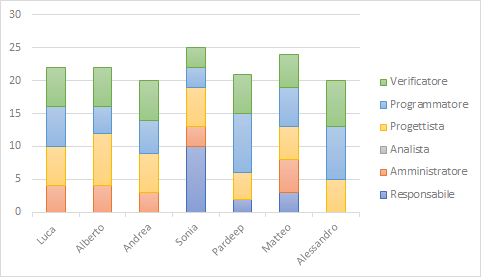
\includegraphics[width=15cm,keepaspectratio]{../includes/pics/grafici/grafico9.png}
	\caption{\label{fig:mission}Distribuzione oraria dei ruoli}
\end{figure}
\clearpage
\subsubsection{Prospetto economico}
Durante il periodo di \markg{validazione} la distribuzione dei ruoli fra i membri del gruppo è stata la seguente:
\begin{center}
	\renewcommand{\arraystretch}{1.5}
	\rowcolors{3}{tableLightYellow}{}
	\begin{longtable}[H]{  	>{\RaggedRight}p{5.6cm}  
							>{\RaggedRight}p{3cm} 
							>{\RaggedRight}p{3cm}  
							}
							
		\rowcolor{tableHeadYellow}
		\textbf{Ruolo}   & \textbf{Ore} & \textbf{Costo (Euro)} \\ 
		\endhead

		Responsabile   & 15   & 450,00 \\
		Amministratore & 19   & 380,00 \\
		Analista       & 0    & 0,00 \\
		Progettista    & 40   & 880,00 \\
		Programmatore  & 41   & 615,00 \\
		Verificatore   & 39   & 585,00 \\
		Totale         & 154  & 2.910,00 \\

		\rowcolor{white}
		\caption{Tabella prospetto economico}
	\end{longtable}
\end{center}
Il seguente grafico mostra visivamente la distribuzione dei ruoli:
%(immagine grafico 10)
\begin{figure}[H]
	\centering
	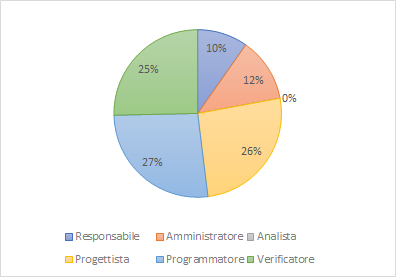
\includegraphics[width=15cm,keepaspectratio]{../includes/pics/grafici/grafico10.png}
	\caption{\label{fig:mission}Divisione dei ruoli tra i membri}
\end{figure}
\clearpage
\subsection{Totale ore rendicontate}
\label{sec:totale_ore}
\subsubsection{Totale suddivisione ore rendicontate}
Di seguito viene riportato il totale delle ore rendicontane nel preventivo a carico del committente:
\begin{center}
	\renewcommand{\arraystretch}{1.5}
	\rowcolors{3}{tableLightYellow}{}
	\begin{longtable}[H]{ 	>{\RaggedRight}p{3.5cm}  
							>{\Centering}p{1.2cm} 
							>{\Centering}p{1.2cm}  
							>{\Centering}p{1.2cm} 
							>{\Centering}p{1.2cm}  
							>{\Centering}p{1.2cm} 
							>{\Centering}p{1.2cm}  
							>{\Centering}p{1.4cm}  
							}
							
		\rowcolor{tableHeadYellow}
		\textbf{Nome}   & \textbf{Re} & \textbf{Ad} & \textbf{An} & \textbf{Pj} & \textbf{Pr} & \textbf{Ve} & \textbf{TOT} \\ 
		\endhead

		Luca Stocco       & 7   & 8    & 2   & 30   & 27    & 26   &   100 \\  
		Alberto Miola     & 5   & 9     & 4   & 31   & 27    & 24   &   100 \\  
		Andrea Pavin      & 6   & 10    & 3   & 28   & 27    & 26   &   100 \\  
		Sonia Menon       & 10  & 7     & 2   & 28   & 27    & 26   &   100 \\  
		Pardeep Singh     & 5   & 7     & 4   & 30   & 28    & 26   &   100 \\  
		Matteo Pellanda   & 6   & 9     & 5   & 29   & 27    & 24   &   100 \\
		Alessandro Pegoraro & 7 & 7		& 5	  & 29	 & 27 	& 25 	& 100\\   

		\rowcolor{white}
		\caption{Tabella suddivisione ore rendicontate}
	\end{longtable}
\end{center}
Il seguente grafico mostra visivamente la distribuzione dei ruoli:
%(immagine grafico 11)
\begin{figure}[H]
	\centering
	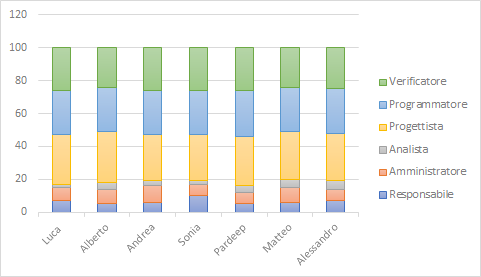
\includegraphics[width=15cm,keepaspectratio]{../includes/pics/grafici/grafico11.png}
	\caption{\label{fig:mission}Distribuzione oraria dei ruoli}
\end{figure}
\clearpage
\subsubsection{Totale prospetto economico rendicontato}
\begin{center}
	\renewcommand{\arraystretch}{1.5}
	\rowcolors{3}{tableLightYellow}{}
	\begin{longtable}[H]{  	>{\RaggedRight}p{5.6cm}  
							>{\RaggedRight}p{3cm} 
							>{\RaggedRight}p{3cm}  
							}

		\rowcolor{tableHeadYellow}
		\textbf{Ruolo}   & \textbf{Ore} & \textbf{Costo (Euro)} \\ 
		\endhead

		Responsabile   & 46    & 1.380,00 \\
		Amministratore & 57    & 1.140,00 \\
		Analista       & 25    & 625,00 \\
		Progettista    & 205   & 4.510,00 \\
		Programmatore  & 184   & 2.760,00 \\
		Verificatore   & 178   & 2.670,00 \\
		Totale         & 695   & 13.085,00 \\

		\rowcolor{white}
		\caption{Tabella prospetto economico rendicontato}
	\end{longtable}
\end{center}
Il seguente grafico mostra visivamente la distribuzione dei ruoli:
%(immagine grafico 12)
\begin{figure}[H]
	\centering
	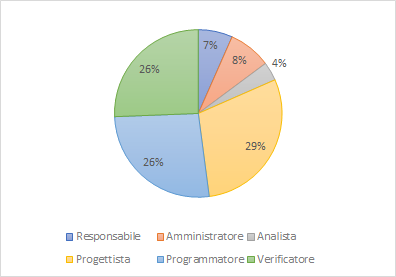
\includegraphics[width=15cm,keepaspectratio]{../includes/pics/grafici/grafico12.png}
	\caption{\label{fig:mission}Divisione dei ruoli tra i membri}
\end{figure}
